Los resultados obtenidos en cada uno de los pasos de este trabajo se detallan en
este capítulo, comenzando por el motor obtenido en la primer iteración de
optimización con el algoritmo genético junto con el modelo de CAD generado.
%
Luego se muestran los resultados de las flujometrías realizadas a partir del
modelo de CAD, incluyendo las mallas obtenidas para algunos casos seleccionados
y el resultado detallado de algunas de las flujometrías, finalizando con el mapa
de $C_{D}$ obtenido, tanto para el puerto de admisión como para
el puerto de escape.

Por último se presentan los resultados de la segunda ronda de optimización con
el algoritmo genético, en la que se utilizó el mapa de $C_{D}$ obtenido en el
paso previo.

\section{Primer Iteración}
%
La primer optimización se realizó partiendo de una población al azar, con los
coeficientes de descarga constantes de 0.7 y 0.75 para el puerto de admisión y
escape respectivamente.
%
El algoritmo genético se ejecutó durante 100 generaciones con una población de
100 individuos y la función objetivo definida en la
sección~\ref{sec:funcion_objetivo} con los pesos indicados, operadores y
parámetros correspondientes indicados en la tabla~\ref{tab:config_genetico}.

\begin{table}[ht!]
  \centering
  \begin{tabular}{cc} \toprule
    Parámetro & Valor \\ \midrule
    RPMS & $1000\times[1, 2, 3, 4, 5, 6, 7, 8, 9]$ \\
    Pesos de función objetivo & $(1, 1, 1, 6, 8, 9, 8, 7, 7)$ \\
    Cantidad de ciclos de ICESym & 2 \\
    Diámetro mínimo & 0.05 \\
    Diámetro máximo & 0.1 \\
    Longitud mínima de tubo & 0.5 \\
    Longitud máxima de tubo & 2 \\
    Ángulo mínimo & 0 \\
    Ángulo máximo & 90 \\
    Separación angular máxima & 70 \\
    Tamaño de población & 100 \\
    Tamaño de torneo & 10 \\
    $\mu$ & 0 \\
    $\sigma$ & 1 \\
    $\alpha$ & 0.5 \\
    Probabilidad de cruza & 0.9 \\
    Probabilidad de mutación & 0.5 \\
    Cantidad de generaciones & 20 \\
    Tamaño de \emph{SALÓN DE LA FAMA} & 1 \\ \bottomrule
    \end{tabular}
  \caption{Configuración utilizada.}\label{tab:config_genetico}
\end{table}

% Para ICESym se utilizaron dos ciclos de simulación, por considerarse que es
% suficientemente preciso para esta primer aproximación.
% %
% En la figura XX se puede ver que a partir de la segunda iteración se obtienen
% buenos resultados, esto se debe a que los datos de partida para la segunda
% iteración, son los resultados de la primer iteración.
%
%
%

En la gráfica de evolución se observa  que se obtuvo rápidamente un individuo
con un puntaje relativamente alto en en las primeras iteraciones, el resultado
final tiene una aptitud 1.5 veces la aptitud media de la población de la última
generación, los parámetros que definen este candidato son los listados en la
tabla y se ilustran en la figura~\ref{fig:primer_op}.
%
Este motor tiene un rendimiento volumétrico máximo de $r_{v} \simeq 0.83$ para 2500
RPM y si bien la función objetivo favorece curvas suaves, se ven dos picos de
rendimiento en la curva, siendo el segundo con $r_{v} \simeq 0.79$ a 7500 RPM.

\begin{figure}
\begin{center}
  \begin{tabular}{rl}
    \begin{tikzpicture}[baseline, trim axis left]
      \begin{axis}[
        xlabel=Generación,
        ylabel=Puntaje,
    legend pos=south east,
        grid=both,
        ]
        \addplot table [x=Gen,y=Avg]{data/genetico.dat} ;
        \addplot table [x=Gen,y=Max]{data/genetico.dat} ;
        \legend{Media, Máximo}
      \end{axis}
    \end{tikzpicture}
    &
    \begin{tikzpicture}[baseline, trim axis right]
      \begin{axis}[
        xlabel=Velocidad del motor [RPM],
        yticklabel pos=upper,
        ylabel={$\eta_{v},x_{r}$},
        ylabel near ticks,
        grid=both,
        legend pos=south east,
        ]
        \addplot table [x=RPM,y=RendVol]{data/primer_rend_vol.dat} ;
        \addplot table [x=RPM,y=FracRes]{data/primer_rend_vol.dat} ;
        \legend{$\eta_{v}$, $x_{r}$ }
      \end{axis}
    \end{tikzpicture}
    \\
  \end{tabular}
\end{center}
\caption{Primer Iteración} \label{fig:primer_op}
\end{figure}

\begin{table}
  \centering
  \begin{tabular}{ccc} \toprule
    Parámetro & Valor & Unidad \\ \midrule
    DTA & 97.24 & mm\\
    DTE & 81.15 & mm\\
    LIT & 519.31 & mm\\
    LET & 976.66 & mm\\
    IIA & 1.12 & grado\\
    IFA & 70.15 & grado\\
    EIA & 85.14 & grado\\
    EFA & 11.13 & grado\\ \bottomrule
  \end{tabular}
  \caption{Mejor Candidato.}\label{tab:resultado_primer_it}
\end{table}

En la figura~\ref{fig:PoTi_primer_op} se muestran las curvas de potencia y
torque del motor, como es de esperarse se ve que ambas copian la curva de
rendimiento volumétrico, con una potencia indicada máxima de 230 HP a 9000 rpm y
un torque máximo de 210 N.m. a\ 7500 RPM.
NOTA: FALTA CORREGIR ESTA POTENCIA CON EL MODELO DE FLOR O DE KNOLL
% TODO
% NOTA: FALTA CORREGIR ESTA POTENCIA CON EL MODELO DE FLOR O DE KNOLL

\begin{figure}
  \begin{center}
  \begin{tikzpicture}
    \begin{axis}[
      xlabel=Velocidad del motor [RPM],
      ylabel={$P_{i}[HP],T_{i}[N.m.]$},
  legend pos=south east,
      grid=both,
      width={13cm}]
      \addplot table [x=RPM,y=PotInd]{data/primer_rend_vol.dat} ;
      \addplot table [x=RPM,y=PotNet]{data/primer_rend_vol.dat} ;
      \addplot table [x=RPM,y=TorqInd]{data/primer_rend_vol.dat} ;
      \addplot table [x=RPM,y=TorqNet]{data/primer_rend_vol.dat} ;
      \legend{Potencia Indicada, Potencia Neta, Torque Indicado, Torque Neto}
      \legend{$\dot{W}_{i,n,1}$,$\dot{W}_{freno,1}$ , $T_{i,1}$, $T_{freno,1}$}
    \end{axis}
  \end{tikzpicture}
  \end{center}
  \caption{Torque y Potencia de Primer Iteración} \label{fig:PoTi_primer_op}
\end{figure}


\section{Modelo de CAD}
%
A partir de los resultados obtenidos se realizó un modelo de CAD de los puertos
que se ilustra en la figura~\ref{fig:motor_cad1} y~\ref{fig:motor_cad2}.
%
Se representó solamente la mitad superior del motor que contiene ambos puertos
de admisión y escape, este modelo es paramétrico y permite rotar los componentes
del motor para obtener distintas posiciones del conjunto para generar la
geometría a evaluar.

% Algunos redondearon las aristas internas incluyendo las paletas y las puntas del rotor para favorecer el proceso de mallado, ya que los bordes agudos pueden ser problmeáticos para el mallador \emph{snappyHexMesh}.

\begin{figure}[ht]
  \centering
    \begin{subfigure}{0.4\textwidth}
        \centering
        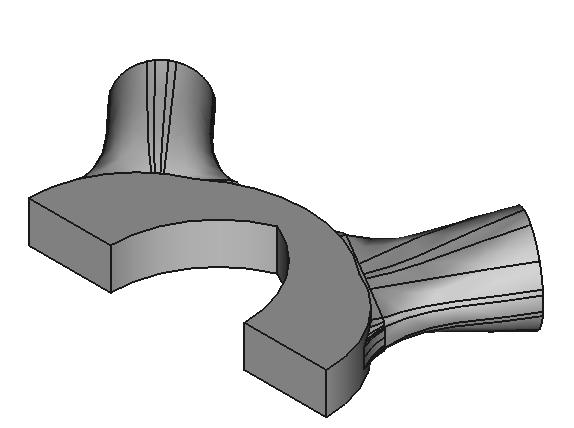
\includegraphics[width=\textwidth]{CAD/motor_cad1.png}
    \end{subfigure}
    \hfill
    \begin{subfigure}{0.4\textwidth}
        \centering
        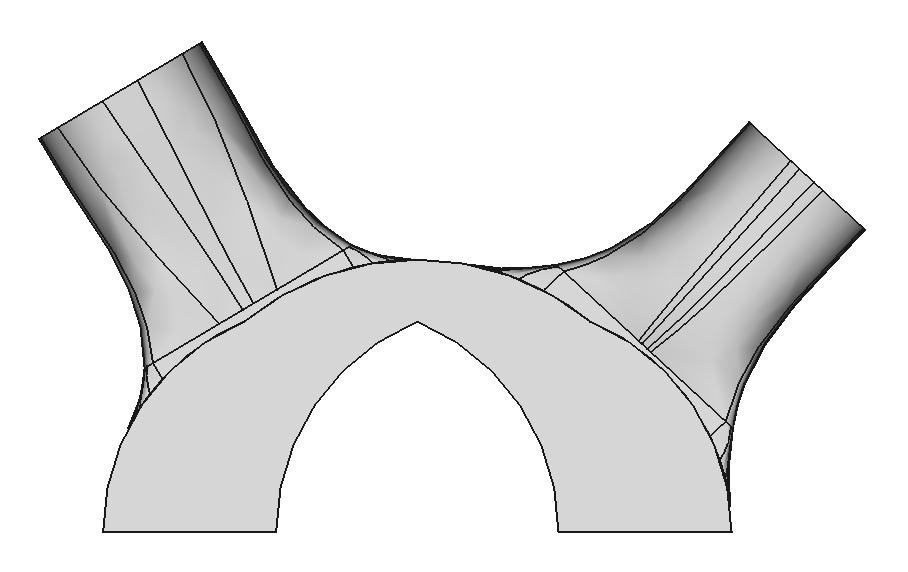
\includegraphics[width=\textwidth]{CAD/motor_cad2.png}
    \end{subfigure}
  \caption{CAD Primer Iteración}\label{fig:motor_cad1}
\end{figure}


\begin{figure}[ht]
  \centering
    \begin{subfigure}{0.8\textwidth}
        \centering
        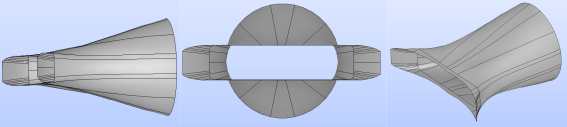
\includegraphics[width=\textwidth]{CAD/vistas_admision.png}
        \caption{Puerto de Admsisión.}
    \end{subfigure}
    \begin{subfigure}{0.8\textwidth}
        \centering
        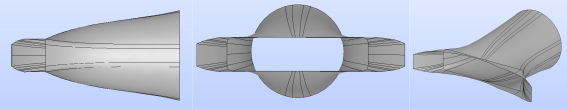
\includegraphics[width=\textwidth]{CAD/vistas_escape.png}
        \caption{Puerto de Escape.}
    \end{subfigure}
  \caption{CAD Primer iteración (vistas fuera de escala).}\label{fig:motor_cad2}
\end{figure}

La altura del puerto del lado de la cámara de combustión se mantuvo en dos
tercios del a altura de cámara $h_{p} = \frac{2}{3}h_{c}$, manteniendo el eje
central de cada puerto de forma que intersecte el centro del motor con el
propósito de eliminar una variable de la geometŕia a modelar.
%
El foco de esta etapa de optimización es el diámetro del puerto y el reglaje.
%
% Se generó uno de estos modelos para cada posición del cigueñal simulada en las
% fluojmetrías.

%%%%%%%%%%%%%%%%%%%%%%%%%%%%%%%%%%%%%%%%%%%%%%%%%%%%%%%%%%%%%%%%%%%%%%%%%%%%%%%
